%%%%%%%%%%%%%%%%%%%%%%%%%%%%%%%%%%%%%%%%%%%%%%%%%%%%%%%%%%%%%%%%%%%%%%%
%% Main Document
%%%%%%%%%%%%%%%%%%%%%%%%%%%%%%%%%%%%%%%%%%%%%%%%%%%%%%%%%%%%%%%%%%%%%%%
\documentclass[a4paper,11pt]{article}

%%%%%%%%%%%%%%%%%%%%%%%%%%%%%%%%%%%%%%%%%%%%%%%%%%%%%%%%%%%%%%%%%%%%%%%
%% EIT Package and Language Settings
%%%%%%%%%%%%%%%%%%%%%%%%%%%%%%%%%%%%%%%%%%%%%%%%%%%%%%%%%%%%%%%%%%%%%%%

% font is RedHatText from RPTU Brand Design
% use [de] option for German documents
%\usepackage{style-eit-latex/EIT}
\usepackage[de]{style-eit-latex/EIT}

%%%%%%%%%%%%%%%%%%%%%%%%%%%%%%%%%%%%%%%%%%%%%%%%%%%%%%%%%%%%%%%%%%%%%%%
%% Custom Packages
%%%%%%%%%%%%%%%%%%%%%%%%%%%%%%%%%%%%%%%%%%%%%%%%%%%%%%%%%%%%%%%%%%%%%%%

% TODO: add own packages here
%\usepackage[european]{circuitikz}		% Circuitikz-Umgebung (Schaltungen)
\usepackage{tikz}						% Tikz-Umgebung
\usepackage{epstopdf}					% Einbinden von EPS-Dateien
\usepackage[figurename=Abb.,tablename=Tab.,justification=centering]{caption}	% Damit "Abb." statt "Abbildung" und "Tab." statt "Tabelle"
\usepackage[printonlyused]{acronym}		% Abkürzungsverzeichnis
\usepackage{color}						% wird für .pdf_tex benötigt
\usepackage{transparent}				% wird für .pdf_tex benötigt
\usepackage{subcaption}

\newcommand\RPTULogo{%
\put(86,716){%
\parbox[b][5cm]{\textwidth}{%
\centering
\begin{tabularx}{\textwidth}{@{}lXr@{}}
\savecellbox{
\includegraphics[width=0.385\textwidth]{style-eit-latex/backgrounds/RPTU_Logo_1c-1_dunkelblau.pdf}} & & 
\savecellbox{
\includegraphics[scale=0.5]{style-eit-latex/backgrounds/Lehrstuhllogo.pdf}} \\ % Hier das Lehrstuhllogo einbinden
[-\rowheight] \printcellmiddle & & \printcellmiddle \\ 
\end{tabularx}
}}}

%%%%%%%%%%%%%%%%%%%%%%%%%%%%%%%%%%%%%%%%%%%%%%%%%%%%%%%%%%%%%%%%%%%%%%%
%% Hyphenation
%%%%%%%%%%%%%%%%%%%%%%%%%%%%%%%%%%%%%%%%%%%%%%%%%%%%%%%%%%%%%%%%%%%%%%%

% correct bad hyphenation here
\hyphenation{
	Re-gion 
	Kurz-name 
	Wind-ener-gie
}

%%%%%%%%%%%%%%%%%%%%%%%%%%%%%%%%%%%%%%%%%%%%%%%%%%%%%%%%%%%%%%%%%%%%%%%
%% Document Configuration
%%%%%%%%%%%%%%%%%%%%%%%%%%%%%%%%%%%%%%%%%%%%%%%%%%%%%%%%%%%%%%%%%%%%%%%
% import global settings file
%%%%%%%%%%%%%%%%%%%%%%%%%%%%%%%%%%%%%%%%%%%%%%%%%%%%%%%%%%%%%%%%%%%%%%%
%% Global Document Settings
%%%%%%%%%%%%%%%%%%%%%%%%%%%%%%%%%%%%%%%%%%%%%%%%%%%%%%%%%%%%%%%%%%%%%%


%%%%%%%%%%%%%%%%%%%%%%%%%%%%%%%%%%%%%%%%%%%%%%%%%%%%%%%%%%%%%%%%%%%%%%%
%% Headers & Footers
%%%%%%%%%%%%%%%%%%%%%%%%%%%%%%%%%%%%%%%%%%%%%%%%%%%%%%%%%%%%%%%%%%%%%%

% page style for front page
\fancypagestyle{frontpage}{
	\fancyhf{}
	
	%remove top line
	\renewcommand{\headrulewidth}{0pt}

	\fancyfoot[L]{
		\color{black} \footnotesize
	}
	\fancyfoot[C]{
		\color{black} \footnotesize
	}
	\fancyfoot[R]{
		\color{black} \footnotesize
		\iftoggle{isGerman}{
  			Seite \thepage
		}{
			Page \thepage
		}
	}
}

% page style for all other pages
\fancypagestyle{otherpages}{
	
	\fancyhf{}

	%remove top line
	%\renewcommand{\headrulewidth}{0pt}

	\fancyhead[L]{\nouppercase{\leftmark}
		\color{black} \footnotesize
	}
	\fancyhead[C]{
		\color{black} \footnotesize
	}
	\fancyhead[R]{
		\color{black} \footnotesize
	}

	\fancyfoot[L]{
		\color{black} \footnotesize
	}
	\fancyfoot[C]{
		\color{black} \footnotesize
	}
	\fancyfoot[R]{
		\color{black} \footnotesize
		\iftoggle{isGerman}{
  			Seite \thepage
		}{
			Page \thepage
		}
	}
}

\fancypagestyle{firstsection}{%
	\fancyhf{}%
	
	\fancyhead[L]{
		\color{black} \footnotesize
	}
	\fancyhead[C]{
		\color{black} \footnotesize
	}
	\fancyhead[R]{
		\color{black} \footnotesize
	}
	
	\fancyfoot[L]{
		\color{black} \footnotesize
	}
	\fancyfoot[C]{
		\color{black} \footnotesize
	}
	\fancyfoot[R]{
		\color{black} \footnotesize
		\iftoggle{isGerman}{
			Seite \thepage
		}{
			Page \thepage
		}
	}
}


% standard page style except for frontpage
\pagestyle{otherpages}



%%%%%%%%%%%%%%%%%%%%%%%%%%%%%%%%%%%%%%%%%%%%%%%%%%%%%%%%%%%%%%%%%%%%%%%
%% Glossaries
%%%%%%%%%%%%%%%%%%%%%%%%%%%%%%%%%%%%%%%%%%%%%%%%%%%%%%%%%%%%%%%%%%%%%%
\usepackage{siunitx}
\usepackage[acronym,symbols,nogroupskip]{glossaries-extra}

%\setlength{\glsdescwidth}{.72\textwidth}

% new keys must be defined before use
\glsaddstoragekey{unit}{}{\glsentryunit}
\glsnoexpandfields

% Style für Glossar
\newglossaryentry{anthropogen}
{
	type=main,
	name=anthropogen,
	description={Der Begriff bezeichnet etwas, was durch den Menschen verursacht oder beeinflusst wird. Im Kontext des Klimawandels beschreibt der Begriff den Einfluss des Menschen auf das Klima der Erde.}
} % Glossareinträge hier einfügen

\newglossarystyle{glossar}{%
	\setglossarystyle{long3col}% base this style on the list style
	\renewenvironment{theglossary}{% Change the table type --> 3 columns
		\begin{longtable}{|p{.17\textwidth}|p{.774\textwidth}|}}%
		{\end{longtable}}%
	%
	\renewcommand*{\glossaryheader}{%  Change the table header
		\hline \bfseries Begriff & \bfseries Beschreibung  \\\hline
		\endhead}%
	\renewcommand*{\glossentry}[2]{%  Change the displayed items
		\glstarget{##1}{\glossentryname{##1}} %
		& \glossentrydesc{##1}% Description
		\tabularnewline \hline
	}%
}

% Style für Abkürzungsverzeichnis
% verwendete Abkürzungen

\newacronym{bmwi}{BMWI}{Bundesministerium für Wirtschaft und Energie}
\newacronym{ch4}{\ensuremath{\text{CH}_{\text{4}}}}{Methan}
\newacronym{co2}{\ensuremath{\text{CO}_{\text{2}}}}{Kohlenstoffdioxid}
\newacronym{ml}{ML}{Maschinelles Lernen}
\newacronym{nh3}{\ensuremath{\text{NH}_{\text{3}}}}{Ammoniak}
\newacronym{thg}{THG}{Treibhausgas}

%%%%%%%%%%%%%%%%%%%%%%%%%%%%%%%%%%%%%%%%%%%%%%%%%%%%%%%%%%%%%%%%%%%%%%%%%%%%%%
% example
%%%%%%%%%%%%%%%%%%%%%%%%%%%%%%%%%%%%%%%%%%%%%%%%%%%%%%%%%%%%%%%%%%%%%%%%%%%%%%

% \newacronym{utc}{UTC}{Coordinated Universal Time}
% \newacronym{adt}{ADT}{Atlantic Daylight Time}
% \newacronym{est}{EST}{Eastern Standard Time}

% Reference acronyms: \gls{UTC}

% Don’t use \gls in chapter or section headings as it can have some unpleasant side-effects. Instead use \glsentrytext for regular entries and one of \glsentryshort, \glsentryshortpl, \glsentrylong, \glsentrylongpl or \glsentryfull for acronyms. Alternatively use glossaries-extra which provides special commands for use in section headings and captions, such as \glsfmtshort{<label>}.
% http://tug.ctan.org/macros/latex/contrib/glossaries/glossariesbegin.pdf % Abkürzungen hier einfügen

\NewEnviron{acronymtable}{%
    \begin{xltabular}{\textwidth}{|c|X|}%
        \BODY
    \end{xltabular}
}
\newglossarystyle{acronyms}{%
	\setglossarystyle{long3col}% base this style on the list style
	\renewenvironment{theglossary}{% Change the table type --> 3 columns
    \acronymtable
    }{
    \endacronymtable
    }
	%
	\renewcommand*{\glossaryheader}{%  Change the table header
		\hline \bfseries Abkürzung & \bfseries Bedeutung  \\\hline
		\endhead}%
	\renewcommand*{\glossentry}[2]{%  Change the displayed items
		\glstarget{##1}{\glossentryname{##1}} %
		& \glossentrydesc{##1}% Description
		  \tabularnewline \hline
	}%
}

% Style für Symbolverzeichnis
% verwendete Symbole

% example
\glsxtrnewsymbol[description={Strom},unit={\si{$\mathrm{\ampere}$}}]{I}{\ensuremath{I}}
\glsxtrnewsymbol[description={Spannung},unit={\si{$\mathrm{\volt}$}}]{U}{\ensuremath{U}} % Symbole hier einfügen

\NewEnviron{symboltable}{%
    \begin{xltabular}{\textwidth}{|c|X|c|}%
        \BODY
    \end{xltabular}
}
\newglossarystyle{symbunitlong}{%
	\setglossarystyle{long3col}% base this style on the list style
	\renewenvironment{theglossary}{%
    \symboltable
    }{
    \endsymboltable
    }
	\renewcommand*{\glossaryheader}{%  Change the table header
		\hline \bfseries Variable & \bfseries Bedeutung & \bfseries Basiseinheit\\\hline
		\endhead}%
	\renewcommand*{\glossentry}[2]{%  Change the displayed items
		\glstarget{##1}{\glossentryname{##1}} %
		& \glossentrydesc{##1}% Description
		& \glsentryunit{##1}  \tabularnewline \hline
	}%
}

%% glossaries package for list of abbreviations and list of symbols
%\usepackage{datatool} % package needed by glossaries
%\usepackage[acronym]{glossaries} % *after* hyperref
%\newglossary[symlog]{symbol}{symi}{symo}{Symbols}
%\makeglossaries
%\glstoctrue
%\input{../../paper.library/abbreviations_symbols/abbreviations}
%\input{../../paper.library/abbreviations_symbols/symbols_finance}

% TODO: add own settings here
\numberwithin{equation}{section}	% Damit bei Gleichungsnummerierungen die 
									% Kapitelnummer davor steht
\numberwithin{figure}{section}		% Damit bei Abbildungsnummerierungen die 
									% Kapitelnummer davor steht
\numberwithin{table}{section}		% Damit bei Tabellennummerierungen die 
									% Kapitelnummer davor steht

\renewcommand{\baselinestretch}{1.5}

%\graphicspath{{Material/}}			% Festlegen des Pfades der Grafiken (für .pdf_tex Dateien)

%%%%%%%%%%%%%%%%%%%%%%%%%%%%%%%%%%%%%%%%%%%%%%%%%%%%%%%%%%%%%%%%%%%%%%%
%% Title and Document Information
%%%%%%%%%%%%%%%%%%%%%%%%%%%%%%%%%%%%%%%%%%%%%%%%%%%%%%%%%%%%%%%%%%%%%%%
\begin{document}
\AddToShipoutPicture*{\RPTULogo}
\begin{titlepage}

	\newcommand{\HRule}{\rule{\linewidth}{1.5mm}}
	\begin{verbatim}
	


 
	
	
	\end{verbatim}
	\begin{center}
		\textbf{\LARGE{Bachelorarbeit - Masterarbeit}}\\
		\begin{verbatim}
		\end{verbatim}
		\HRule\\[0.4cm]
		
		{\LARGE\bfseries <Titel deutsch>}\\[0.2cm] % Title of your document
		
		\HRule\\[0.5cm]
		\HRule\\[0.4cm]
		
		{\LARGE\bfseries <Title english>}\\[0.2cm] % Title of your document
		
		\HRule\\[1.5cm]
	\end{center}
	
	\begin{verbatim}

	\end{verbatim}
    \begin{center}
		Verfasser: <Verfasser>\\
		Matrikelnummer: <Matrikelnummer>\\

		Abgabedatum: \today
		\\
		
		\vfill
		\begin{tabular}{ll}
			\multicolumn{2}{l}{<Lehrstuhlname>} \\
			Prüfer:     & <Prüfer> \\
			Betreuer:   & <Betreuer>
		\end{tabular}
	\end{center}



\end{titlepage} \label{Deckblatt} % Deckblatt
\ClearShipoutPicture
\pagenumbering{Roman}
\setcounter{page}{2}

%%%%%%%%%%%%%%%%%%%%%%%%%%%%%%%%%%%%%%%%%%%%%%%%%%%%%%%%%%%%%%%%%%%%%%%
%% eidesstattliche Erklärung, Abstract und Inhaltsverzeichnis
%%%%%%%%%%%%%%%%%%%%%%%%%%%%%%%%%%%%%%%%%%%%%%%%%%%%%%%%%%%%%%%%%%%%%%%
\phantomsection
\markboth{Eidesstattliche Erklärung}{Eidesstattliche Erklärung}
\section*{Eidesstattliche Erklärung}
\addcontentsline{toc}{section}{Eidesstattliche Erklärung} 

Ich versichere hiermit an Eides statt, die vorliegende Arbeit gemäß BPO/MPO Elektrotechnik und Informationstechnik bis auf die durch meinen Betreuer gewährte Unterstützung ohne Hilfe Dritter selbstständig angefertigt, alle benutzten Quellen und Hilfsmittel einschließlich des Internets vollständig und genau angegeben und alles kenntlich gemacht zu haben, was aus Arbeiten anderer unverändert, mit Abkürzung oder sinngemäß übernommen wurde.
\begin{verbatim}

\end{verbatim}
Kaiserslautern, den \today
\begin{verbatim}



\end{verbatim}
<Vorname> <Nachname> \label{Eidesstatt} % eidesstattliche Erklärung

\newpage
\phantomsection
\markboth{Kurzfassung | Abstract}{Kurzfassung | Abstract}
\section*{Kurzfassung}
\addcontentsline{toc}{section}{Kurzfassung | Abstract} 
Lorem ipsum dolor sit amet, consetetur sadipscing elitr, sed diam nonumy eirmod tempor invidunt ut labore et dolore magna aliquyam erat, sed diam voluptua. At vero eos et accusam et justo duo dolores et ea rebum. Stet clita kasd gubergren, no sea takimata sanctus est Lorem ipsum dolor sit amet. Lorem ipsum dolor sit amet, consetetur sadipscing elitr, sed diam nonumy eirmod tempor invidunt ut labore et dolore magna aliquyam erat, sed diam voluptua. At vero eos et accusam et justo duo dolores et ea rebum. Stet clita kasd gubergren, no sea takimata sanctus est Lorem ipsum dolor sit amet.

\selectlanguage{english}
\section*{Abstract}
Lorem ipsum dolor sit amet, consetetur sadipscing elitr, sed diam nonumy eirmod tempor invidunt ut labore et dolore magna aliquyam erat, sed diam voluptua. At vero eos et accusam et justo duo dolores et ea rebum. Stet clita kasd gubergren, no sea takimata sanctus est Lorem ipsum dolor sit amet. Lorem ipsum dolor sit amet, consetetur sadipscing elitr, sed diam nonumy eirmod tempor invidunt ut labore et dolore magna aliquyam erat, sed diam voluptua. At vero eos et accusam et justo duo dolores et ea rebum. Stet clita kasd gubergren, no sea takimata sanctus est Lorem ipsum dolor sit amet.

\selectlanguage{ngerman} \label{Abstract} % Abstract

\newpage
\markboth{Inhaltsverzeichnis}{Inhaltsverzeichnis}
\setcounter{tocdepth}{4}
\setcounter{secnumdepth}{4}
\tableofcontents

\newpage
\pagenumbering{arabic}

%%%%%%%%%%%%%%%%%%%%%%%%%%%%%%%%%%%%%%%%%%%%%%%%%%%%%%%%%%%%%%%%%%%%%%%
%% Text
%%%%%%%%%%%%%%%%%%%%%%%%%%%%%%%%%%%%%%%%%%%%%%%%%%%%%%%%%%%%%%%%%%%%%%%

% INSERT YOUR CONTENT HERE:

\section{Einleitung} \label{Einleitung} \thispagestyle{firstsection}
Diese Vorlage entspricht den neuen Regeln des Brand Designs der RPTU.
Hierzu wurde die Vorlage von \url{https://github.com/RPTU-EIT/report-eit-latex} modifiziert.
Im Unterordner \texttt{style-eit-latex} ist die Datei \texttt{EIT.sty} hinterlegt.
In dieser Style-Datei wurden die Farben und die Schriftart auf das RPTU-Design umgestellt.
Aufgrund der notwendigen Verwendung bestimmter Packages wird diese Vorlage nur in LuaLaTex unterstützt!\\
Folgende Schriftarten wurden als Standard integriert:
\begin{table}[ht]
    \label{tab:Standardschriftart}
    \caption{RedHatText-Standardschriftart und ihre Formen}
    \centering
    \footnotesize
    \begin{tabular}{@{}ccc@{}}
    \toprule
    Form            & Name der Schriftart                           & Befehl\\ \midrule
    normal          & RedHatText-Regular                            & - \\
    fett            & \textbf{RedHatText-SemiBold}                  & \verb|\bfseries| oder \verb|\textbf{}|\\
    kursiv          & \textit{RedHatText-Italic}                    & \verb|\itshape| oder \verb|\textit{}|\\
    fett \& kursiv  & \textbf{\textit{RedHatText-SemiBoldItalic}}   & \verb|\bfseries\itshape| oder \verb|\textbf{\textit{}}|\\ \bottomrule
    \end{tabular}
\end{table}

Des Weiteren wurden die anderen verfügbaren RedHatText-Schriftarten integriert:
\begin{table}[ht]
    \label{tab:restliche_Schriftarten}
    \caption{Weitere RedHatText-Schriftarten und ihre Formen}
    \centering
    \footnotesize
    \begin{tabular}{@{}ccc@{}}
    \toprule
    Form                    & Name der Schriftart& Befehl\\ \midrule
    light                   & \fontseries{li}\fontshape{n}\selectfont RedHatText-Light          & \verb|\fontseries{li}\fontshape{n}\selectfont|    \\
    light \& kursiv         & \fontseries{li}\fontshape{it}\selectfont RedHatText-LightItalic   & \verb|\fontseries{li}\fontshape{it}\selectfont|   \\
    medium                  & \fontseries{md}\fontshape{n}\selectfont RedHatText-Medium         & \verb|\fontseries{md}\fontshape{n}\selectfont|    \\
    medium \& kursiv        & \fontseries{md}\fontshape{it}\selectfont RedHatText-MediumItalic  & \verb|\fontseries{md}\fontshape{it}\selectfont|   \\
    extra fett              & \fontseries{bf}\fontshape{n}\selectfont RedHatText-Bold           & \verb|\fontseries{bf}\fontshape{n}\selectfont|    \\
    extra fett \& kursiv    & \fontseries{bf}\fontshape{it}\selectfont RedHatText-BoldItalic    & \verb|\fontseries{bf}\fontshape{it}\selectfont|   \\ \bottomrule
    \end{tabular}
\end{table}

\tcbset{
    frame code={}
    center title,
    left=0pt,
    right=0pt,
    top=0pt,
    bottom=0pt,
    colback=gray!70,
    colframe=white,
    width=30mm,
    enlarge left by=0mm,
    boxsep=0pt,
    arc=0pt,outer arc=0pt,
    }

\clearpage
Die Schriftfarbe kann über den \verb|\textcolor{<Farbe>}{<Text>}| Befehl eingestellt werden.
Folgende Farben stehen zur Verfügung:

\begin{table}[ht]
    \label{tab:Farben}
    \caption{RPTU-Farben}
    \centering
    \footnotesize
    \begin{tabular}{@{}cc@{}}
    \toprule
    Farbe & Befehl\\ \midrule
	\bfseries\textcolor{rptublaugrau}{blaugrau}                           & \verb|\textcolor{rptublaugrau}{blaugrau}|       \\
	\bfseries\textcolor{rptugruengrau}{gruengrau}                         & \verb|\textcolor{rptugruengrau}{gruengrau}|     \\
	\bfseries\textcolor{rptudunkelblau}{dunkelblau}                       & \verb|\textcolor{rptudunkelblau}{dunkelblau}|   \\
	\bfseries\textcolor{rptuhellblau}{hellblau}                           & \verb|\textcolor{rptuhellblau}{hellblau}|       \\
	\bfseries\textcolor{rptudunkelgruen}{dunkelgruen}                     & \verb|\textcolor{rptudunkelgruen}{dunkelgruen}| \\
	\bfseries\textcolor{rptuhellgruen}{hellgruen}                         & \verb|\textcolor{rptuhellgruen}{hellgruen}|     \\
	\bfseries\textcolor{rptuviolett}{violett}                             & \verb|\textcolor{rptuviolett}{violett}|         \\
	\bfseries\textcolor{rptupink}{pink}                                   & \verb|\textcolor{rptupink}{pink}|               \\
	\bfseries\textcolor{rpturot}{rot}                                     & \verb|\textcolor{rpturot}{rot}|                 \\
	\bfseries\textcolor{rptuorange}{orange}                               & \verb|\textcolor{rptuorange}{orange}|           \\
	\bfseries\textcolor{rptuschwarz}{schwarz}                             & \verb|\textcolor{rptuschwarz}{schwarz}|         \\
	\bfseries\begin{tcolorbox}\centering\textcolor{rptuweiss}{weiss}\end{tcolorbox} & \verb|\textcolor{rptuweiss}{weiss}|   \\ \bottomrule
    \end{tabular}
\end{table}

\clearpage % Einleitung

\newpage
\graphicspath{{Kapitel_2/}}
\section{Kapitel 2} \label{sec:Kapitel_2} \thispagestyle{firstsection}
\subsection{Kapitel 2.1} \label{sec:2_1}

\subsubsection{Formeln}\label{sec:2_1_1}
Es empfiehlt sich, Formeln in der folgenden Form anzugeben, damit alle verwendeten Größen nachvollziehbar sind:

\begin{figure}[ht]
    \begin{align}
        y & = a_0 + a_1x \label{eq:linear-Spline}\\
        y & = a_0 + a_1x + a_2x^2 + a_3x^3 \label{eq:cubic-Spline}
    \end{align}
    \footnotesize
    \begin{tabular}{ll}
    $y$   & Funktionswert \\
    $x$   & Datenpunkt \\
    $a_i$ & Koeffizienten
    \end{tabular}
    \normalsize
\end{figure}

\subsubsection{Grafiken}\label{sec:2_1_2}
Grafiken können mittels \verb|\includegraphics| eingefügt werden.
\begin{figure}[ht]
    \centering
    
\includegraphics[scale=0.5]{Kap_2/Grafiken/RPTU_Logo_1c-1.png}
    \caption{RPTU Logo als .png}
    \label{fig:Kap_2_1_2_png}
\end{figure}

Alternativ können auch Vektordateien eingefügt werden.
Grafiken aus Inkscape können auch als \texttt{.tex} Datei hinterlegt werden.
Dazu wird eine Vektorgrafik aus Inkscape über die pdf\_tex Option exportiert.
Inkscape exportiert die Grafik als \texttt{.pdf} und hinterlegt den Text in einer \texttt{.pdf\_tex} Datei.
Letztere kann auch als \texttt{.tex} Datei in \LaTeX \ eingebunden werden, wie das folgende Beispiel zeigen soll:
\clearpage

\begin{figure}[ht]
    \centering
    \def\svgwidth{0.6\textwidth}
    %% Creator: Inkscape inkscape 0.92.4, www.inkscape.org
%% PDF/EPS/PS + LaTeX output extension by Johan Engelen, 2010
%% Accompanies image file 'Beispielgrafik.pdf' (pdf, eps, ps)
%%
%% To include the image in your LaTeX document, write
%%   \input{<filename>.pdf_tex}
%%  instead of
%%   \includegraphics{<filename>.pdf}
%% To scale the image, write
%%   \def\svgwidth{<desired width>}
%%   \input{<filename>.pdf_tex}
%%  instead of
%%   \includegraphics[width=<desired width>]{<filename>.pdf}
%%
%% Images with a different path to the parent latex file can
%% be accessed with the `import' package (which may need to be
%% installed) using
%%   \usepackage{import}
%% in the preamble, and then including the image with
%%   \import{<path to file>}{<filename>.pdf_tex}
%% Alternatively, one can specify
%%   \graphicspath{{<path to file>/}}
%% 
%% For more information, please see info/svg-inkscape on CTAN:
%%   http://tug.ctan.org/tex-archive/info/svg-inkscape
%%
\begingroup%
  \makeatletter%
  \providecommand\color[2][]{%
    \errmessage{(Inkscape) Color is used for the text in Inkscape, but the package 'color.sty' is not loaded}%
    \renewcommand\color[2][]{}%
  }%
  \providecommand\transparent[1]{%
    \errmessage{(Inkscape) Transparency is used (non-zero) for the text in Inkscape, but the package 'transparent.sty' is not loaded}%
    \renewcommand\transparent[1]{}%
  }%
  \providecommand\rotatebox[2]{#2}%
  \newcommand*\fsize{\dimexpr\f@size pt\relax}%
  \newcommand*\lineheight[1]{\fontsize{\fsize}{#1\fsize}\selectfont}%
  \ifx\svgwidth\undefined%
    \setlength{\unitlength}{265.58093262bp}%
    \ifx\svgscale\undefined%
      \relax%
    \else%
      \setlength{\unitlength}{\unitlength * \real{\svgscale}}%
    \fi%
  \else%
    \setlength{\unitlength}{\svgwidth}%
  \fi%
  \global\let\svgwidth\undefined%
  \global\let\svgscale\undefined%
  \makeatother%
  \begin{picture}(1,1.05335122)%
    \lineheight{1}%
    \setlength\tabcolsep{0pt}%
	\fontseries{md}\fontshape{n}\selectfont
	\footnotesize
    \put(0,0){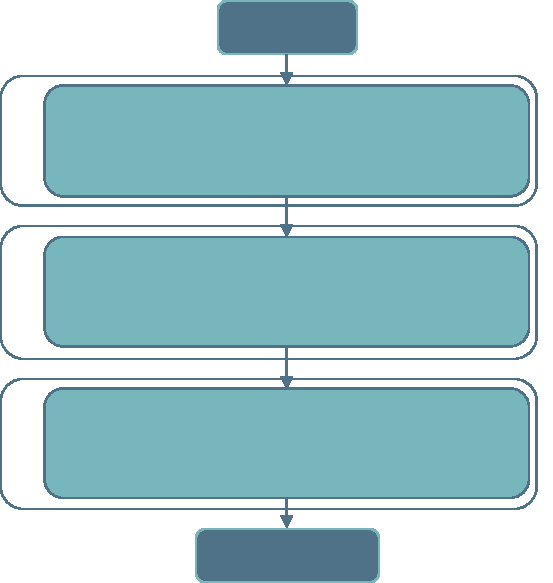
\includegraphics[width=\unitlength,page=1]{Kap_2/Grafiken/Beispielgrafik.pdf}}%
	\put(0.52,0.99404727){\color{rptugruengrau}\makebox(0,0)[ct]{\lineheight{1.25}\smash{\begin{tabular}[t]{c}Start\end{tabular}}}}%
	\put(0.52,0.038){\color{rptugruengrau}\makebox(0,0)[ct]{\lineheight{1.25}\smash{\begin{tabular}[t]{c}Ende\end{tabular}}}}%
	
	\scriptsize
    \put(0.05072458,0.745){\color{rptublaugrau}\rotatebox{90}{\makebox(0,0)[lt]{\lineheight{1.25}\smash{\begin{tabular}[t]{l}Schritt 1\end{tabular}}}}}%
	\put(0.05072458,0.47){\color{rptublaugrau}\rotatebox{90}{\makebox(0,0)[lt]{\lineheight{1.25}\smash{\begin{tabular}[t]{l}Schritt 2\end{tabular}}}}}%
	\put(0.05072458,0.19){\color{rptublaugrau}\rotatebox{90}{\makebox(0,0)[lt]{\lineheight{1.25}\smash{\begin{tabular}[t]{l}Schritt 3\end{tabular}}}}}%
    
	\fontsize{7.5}{7.5}
    \put(0.1,0.83872738){\color{rptublaugrau}\makebox(0,0)[lt]{\lineheight{1.25}\smash{\begin{tabular}[t]{l}•\end{tabular}}}}%
    \put(0.12,0.83872738){\color{rptublaugrau}\makebox(0,0)[lt]{\lineheight{1.25}\smash{\begin{tabular}[t]{l}Dies ist eine Beispielgrafik,\end{tabular}}}}%
    \put(0.1,0.8076634){\color{rptublaugrau}\makebox(0,0)[lt]{\lineheight{1.25}\smash{\begin{tabular}[t]{l}•\end{tabular}}}}%
    \put(0.12,0.8076634){\color{rptublaugrau}\makebox(0,0)[lt]{\lineheight{1.25}\smash{\begin{tabular}[t]{l}die zeigen soll, wie eine pdf Grafik inkl. Text\end{tabular}}}}%
    \put(0.1,0.77659943){\color{rptublaugrau}\makebox(0,0)[lt]{\lineheight{1.25}\smash{\begin{tabular}[t]{l}•\end{tabular}}}}%
    \put(0.12,0.77659943){\color{rptublaugrau}\makebox(0,0)[lt]{\lineheight{1.25}\smash{\begin{tabular}[t]{l}in \LaTeX \ eingebettet werden kann\end{tabular}}}}%
    \put(0.1,0.74553545){\color{rptublaugrau}\makebox(0,0)[lt]{\lineheight{1.25}\smash{\begin{tabular}[t]{l}•\end{tabular}}}}%
    \put(0.12,0.74553545){\color{rptublaugrau}\makebox(0,0)[lt]{\lineheight{1.25}\smash{\begin{tabular}[t]{l}Dabei lässt sich nicht nur die Schrift anpassen\end{tabular}}}}%
    \put(0.1,0.56479958){\color{rptublaugrau}\makebox(0,0)[lt]{\lineheight{1.25}\smash{\begin{tabular}[t]{l}•\end{tabular}}}}%
    \put(0.12,0.56479958){\color{rptublaugrau}\makebox(0,0)[lt]{\lineheight{1.25}\smash{\begin{tabular}[t]{l}Auch die Schriftfarbe,\end{tabular}}}}%
    \put(0.1,0.53373561){\color{rptublaugrau}\makebox(0,0)[lt]{\lineheight{1.25}\smash{\begin{tabular}[t]{l}•\end{tabular}}}}%
    \put(0.12,0.53373561){\color{rptublaugrau}\makebox(0,0)[lt]{\lineheight{1.25}\smash{\begin{tabular}[t]{l}die Schriftgröße,\end{tabular}}}}%
    \put(0.1,0.50267163){\color{rptublaugrau}\makebox(0,0)[lt]{\lineheight{1.25}\smash{\begin{tabular}[t]{l}•\end{tabular}}}}%
    \put(0.12,0.50267163){\color{rptublaugrau}\makebox(0,0)[lt]{\lineheight{1.25}\smash{\begin{tabular}[t]{l}Schriftart\end{tabular}}}}%
    \put(0.1,0.47160765){\color{rptublaugrau}\makebox(0,0)[lt]{\lineheight{1.25}\smash{\begin{tabular}[t]{l}•\end{tabular}}}}%
    \put(0.12,0.47160765){\color{rptublaugrau}\makebox(0,0)[lt]{\lineheight{1.25}\smash{\begin{tabular}[t]{l} und Schriftposition lässt sich anpassen\end{tabular}}}}%
    \put(0.1,0.2767518){\color{rptublaugrau}\makebox(0,0)[lt]{\lineheight{1.25}\smash{\begin{tabular}[t]{l}•\end{tabular}}}}%
    \put(0.12,0.2767518){\color{rptublaugrau}\makebox(0,0)[lt]{\lineheight{1.25}\smash{\begin{tabular}[t]{l}Die Schriftposition wird\end{tabular}}}}%
    \put(0.1,0.24568782){\color{rptublaugrau}\makebox(0,0)[lt]{\lineheight{1.25}\smash{\begin{tabular}[t]{l}•\end{tabular}}}}%
    \put(0.12,0.24568782){\color{rptublaugrau}\makebox(0,0)[lt]{\lineheight{1.25}\smash{\begin{tabular}[t]{l}über Koordinaten eingestellt\end{tabular}}}}%
    \put(0.1,0.21462384){\color{rptublaugrau}\makebox(0,0)[lt]{\lineheight{1.25}\smash{\begin{tabular}[t]{l}•\end{tabular}}}}%
    \put(0.12,0.21462384){\color{rptublaugrau}\makebox(0,0)[lt]{\lineheight{1.25}\smash{\begin{tabular}[t]{l}die Farben über den \texttt{color} Befehl\end{tabular}}}}%

  \end{picture}%
\endgroup%

    \caption{Beispielgrafik mit eingebetteten Text}
    \label{fig:Kap_2_1_2_tex}
\end{figure}

\subsubsection{Literatur}\label{sec:2_1_3}
Literatur wird in der Datei \texttt{Bibliografie.bib} hinterlegt.
Als Zitierstil ist der IEEE-Stil voreingestellt.
Zitiert wird mittels \verb|\cite{}| Befehl.
Dabei lassen sich Seitenangaben über die Optionen dieses Befehls realisieren.
Zum Beispiel\,\cite[S.416ff]{Brokate.2015}: \verb|\cite[S.416ff]{Brokate.2015}|

\subsubsection{Deckblatt}\label{sec:2_1_4}
Auf dem Deckblatt kann das entsprechende Lehrstuhllogo eingepflegt werden.
Dazu muss das Logo im Unterordner \texttt{style-eit-latex/backgrounds} hinterlegt werden.
Die Einstellungen zum Einfügen des Logos finden sich in der \texttt{Main.tex} in Zeile 35.

\clearpage
\subsection{Kapitel 2.2} \label{sec:2_2}

Lorem ipsum dolor sit amet, consetetur sadipscing elitr, sed diam nonumy eirmod tempor invidunt ut labore et dolore magna aliquyam erat, sed diam voluptua. At vero eos et accusam et justo duo dolores et ea rebum. Stet clita kasd gubergren, no sea takimata sanctus est Lorem ipsum dolor sit amet. Lorem ipsum dolor sit amet, consetetur sadipscing elitr, sed diam nonumy eirmod tempor invidunt ut labore et dolore magna aliquyam erat, sed diam voluptua. At vero eos et accusam et justo duo dolores et ea rebum. Stet clita kasd gubergren, no sea takimata sanctus est Lorem ipsum dolor sit amet.


\subsection{Kapitel 2.3} \label{sec:2_3}

Lorem ipsum dolor sit amet, consetetur sadipscing elitr, sed diam nonumy eirmod tempor invidunt ut labore et dolore magna aliquyam erat, sed diam voluptua. At vero eos et accusam et justo duo dolores et ea rebum. Stet clita kasd gubergren, no sea takimata sanctus est Lorem ipsum dolor sit amet. Lorem ipsum dolor sit amet, consetetur sadipscing elitr, sed diam nonumy eirmod tempor invidunt ut labore et dolore magna aliquyam erat, sed diam voluptua. At vero eos et accusam et justo duo dolores et ea rebum. Stet clita kasd gubergren, no sea takimata sanctus est Lorem ipsum dolor sit amet. % Grundlagen

\newpage
\graphicspath{{Kapitel_3/}}
\section{Kapitel 3}\label{sec:3} \thispagestyle{firstsection}
\subsection{Kapitel 3.1} \label{sec:3_1}

Lorem ipsum dolor sit amet, consetetur sadipscing elitr, sed diam nonumy eirmod tempor invidunt ut labore et dolore magna aliquyam erat, sed diam voluptua. At vero eos et accusam et justo duo dolores et ea rebum. Stet clita kasd gubergren, no sea takimata sanctus est Lorem ipsum dolor sit amet. Lorem ipsum dolor sit amet, consetetur sadipscing elitr, sed diam nonumy eirmod tempor invidunt ut labore et dolore magna aliquyam erat, sed diam voluptua. At vero eos et accusam et justo duo dolores et ea rebum. Stet clita kasd gubergren, no sea takimata sanctus est Lorem ipsum dolor sit amet.

\subsection{Kapitel 3.2} \label{sec:3_2}

Lorem ipsum dolor sit amet, consetetur sadipscing elitr, sed diam nonumy eirmod tempor invidunt ut labore et dolore magna aliquyam erat, sed diam voluptua. At vero eos et accusam et justo duo dolores et ea rebum. Stet clita kasd gubergren, no sea takimata sanctus est Lorem ipsum dolor sit amet. Lorem ipsum dolor sit amet, consetetur sadipscing elitr, sed diam nonumy eirmod tempor invidunt ut labore et dolore magna aliquyam erat, sed diam voluptua. At vero eos et accusam et justo duo dolores et ea rebum. Stet clita kasd gubergren, no sea takimata sanctus est Lorem ipsum dolor sit amet.

\subsection{Kapitel 3.3} \label{sec:3_3}

Lorem ipsum dolor sit amet, consetetur sadipscing elitr, sed diam nonumy eirmod tempor invidunt ut labore et dolore magna aliquyam erat, sed diam voluptua. At vero eos et accusam et justo duo dolores et ea rebum. Stet clita kasd gubergren, no sea takimata sanctus est Lorem ipsum dolor sit amet. Lorem ipsum dolor sit amet, consetetur sadipscing elitr, sed diam nonumy eirmod tempor invidunt ut labore et dolore magna aliquyam erat, sed diam voluptua. At vero eos et accusam et justo duo dolores et ea rebum. Stet clita kasd gubergren, no sea takimata sanctus est Lorem ipsum dolor sit amet.

\newpage
\graphicspath{{Kapitel_4/}}
\section{Kapitel 4} \label{sec:4} \thispagestyle{firstsection}
\subsection{Kapitel 4.1} \label{sec:4_1}

Lorem ipsum dolor sit amet, consetetur sadipscing elitr, sed diam nonumy eirmod tempor invidunt ut labore et dolore magna aliquyam erat, sed diam voluptua. At vero eos et accusam et justo duo dolores et ea rebum. Stet clita kasd gubergren, no sea takimata sanctus est Lorem ipsum dolor sit amet. Lorem ipsum dolor sit amet, consetetur sadipscing elitr, sed diam nonumy eirmod tempor invidunt ut labore et dolore magna aliquyam erat, sed diam voluptua. At vero eos et accusam et justo duo dolores et ea rebum. Stet clita kasd gubergren, no sea takimata sanctus est Lorem ipsum dolor sit amet.

\subsection{Kapitel 4.2} \label{sec:4_2}

Lorem ipsum dolor sit amet, consetetur sadipscing elitr, sed diam nonumy eirmod tempor invidunt ut labore et dolore magna aliquyam erat, sed diam voluptua. At vero eos et accusam et justo duo dolores et ea rebum. Stet clita kasd gubergren, no sea takimata sanctus est Lorem ipsum dolor sit amet. Lorem ipsum dolor sit amet, consetetur sadipscing elitr, sed diam nonumy eirmod tempor invidunt ut labore et dolore magna aliquyam erat, sed diam voluptua. At vero eos et accusam et justo duo dolores et ea rebum. Stet clita kasd gubergren, no sea takimata sanctus est Lorem ipsum dolor sit amet.

\subsection{Kapitel 4.3} \label{sec:4_3}

Lorem ipsum dolor sit amet, consetetur sadipscing elitr, sed diam nonumy eirmod tempor invidunt ut labore et dolore magna aliquyam erat, sed diam voluptua. At vero eos et accusam et justo duo dolores et ea rebum. Stet clita kasd gubergren, no sea takimata sanctus est Lorem ipsum dolor sit amet. Lorem ipsum dolor sit amet, consetetur sadipscing elitr, sed diam nonumy eirmod tempor invidunt ut labore et dolore magna aliquyam erat, sed diam voluptua. At vero eos et accusam et justo duo dolores et ea rebum. Stet clita kasd gubergren, no sea takimata sanctus est Lorem ipsum dolor sit amet.

\newpage

\section{Schlussfolgerung und Ausblick} \label{sec:Fazit} \thispagestyle{firstsection}
Lorem ipsum dolor sit amet, consetetur sadipscing elitr, sed diam nonumy eirmod tempor invidunt ut labore et dolore magna aliquyam erat, sed diam voluptua. At vero eos et accusam et justo duo dolores et ea rebum. Stet clita kasd gubergren, no sea takimata sanctus est Lorem ipsum dolor sit amet. Lorem ipsum dolor sit amet, consetetur sadipscing elitr, sed diam nonumy eirmod tempor invidunt ut labore et dolore magna aliquyam erat, sed diam voluptua. At vero eos et accusam et justo duo dolores et ea rebum. Stet clita kasd gubergren, no sea takimata sanctus est Lorem ipsum dolor sit amet.

%%%%%%%%%%%%%%%%%%%%%%%%%%%%%%%%%%%%%%%%%%%%%%%%%%%%%%%%%%%%%%%%%%%%%%%
%% Verzeichnisse und Anhang
%%%%%%%%%%%%%%%%%%%%%%%%%%%%%%%%%%%%%%%%%%%%%%%%%%%%%%%%%%%%%%%%%%%%%%%

\newpage
\markboth{Literaturverzeichnis}{Literaturverzeichnis}
\thispagestyle{firstsection}
\renewcommand{\refname}{Literaturverzeichnis}
\bibliography{Bibliografie}
\bibliographystyle{deIEEEtran}
\addcontentsline{toc}{section}{Literaturverzeichnis}

\newpage
% Abkürzungen sind in abkuerzungen.tex hinterlegt
\thispagestyle{firstsection}
\printunsrtglossary[title={Abkürzungsverzeichnis},type=acronym,style=acronyms] % Abkürzungsverzeichnis

\newpage
% Symbole sind in symbole.tex hinterlegt
\thispagestyle{firstsection}
\printunsrtglossary[title={Symbolverzeichnis},type=symbols,style=symbunitlong] % Symbolverzeichnis

\newpage
% Glossareinträge sind in glossar.tex hinterlegt
\thispagestyle{firstsection}
\printunsrtglossary[title={Glossar},type=main,style=glossar] % Glossar

\newpage
\phantomsection
\markboth{Tabellenverzeichnis}{Tabellenverzeichnis}
\thispagestyle{firstsection}
\listoftables
\addcontentsline{toc}{section}{Tabellenverzeichnis}

\newpage
\phantomsection
\markboth{Abbildungsverzeichnis}{Abbildungsverzeichnis}
\thispagestyle{firstsection}
\listoffigures
\addcontentsline{toc}{section}{Abbildungsverzeichnis}

\newpage
\phantomsection
\appendix
\markboth{Anhang}{Anhang}
\thispagestyle{firstsection}
\section*{Anhang}
\addcontentsline{toc}{section}{Anhang} 
\setcounter{section}{1}
\setcounter{table}{0}
\subsection{Anhang 1} \label{anh:gzf}
 % Anhang


\end{document}